\documentclass[11pt]{article}
\usepackage[T1]{fontenc}
\usepackage[utf8]{inputenc}
\usepackage{lmodern,amsmath,amssymb,amsthm,mathtools}
\usepackage[margin=1in]{geometry}
\usepackage{booktabs,longtable,array,enumitem,microtype,xcolor}
\usepackage{graphicx,tikz,fancyhdr,listings}
\usepackage[colorlinks=true,linkcolor=blue!45!black,citecolor=blue!45!black,urlcolor=blue!55!black,breaklinks=true]{hyperref}
\hypersetup{pdftitle={Affine Geometry and Paid Recursion for Subexponential SAT},pdfauthor={Research prepared for Vladimir Reshetnikov},pdfsubject={A smaller certified contraction exponent; review of the latest ProveIt packets and Anthropic formalization}}
\newtheorem{theorem}{Theorem}[section]
\newtheorem{lemma}[theorem]{Lemma}
\newtheorem{proposition}[theorem]{Proposition}
\newtheorem{corollary}[theorem]{Corollary}
\theoremstyle{remark}\newtheorem{remark}[theorem]{Remark}
\newcommand{\poly}{\operatorname{poly}}
\newcommand{\pc}{\operatorname{popcount}}
\newcommand{\F}{\mathbb F}
\newcommand{\K}{\mathcal K}
\newcommand{\kap}{\kappa}
\newcommand{\Escale}{\mathcal E}
\newcommand{\pin}{\texttt{73dfb5e5ab6e91bd7375e5b97ef85d7e1cc8e81d}}
\setlength{\emergencystretch}{3em}
\setlength{\headheight}{14pt}
\setlist{itemsep=3pt,topsep=5pt}
\makeatletter
\renewcommand*\l@section[2]{\@dottedtocline{1}{0em}{1.5em}{\bfseries #1}{\bfseries #2}}
\makeatother
\pagestyle{fancy}\fancyhf{}
\fancyhead[L]{\small Affine geometry and paid recursion}
\fancyhead[R]{\small Subexponential SAT research}
\fancyfoot[C]{\thepage}
\lstset{basicstyle=\ttfamily\small,columns=fullflexible,breaklines=true,frame=single,framerule=.3pt}
\title{Affine Geometry and Paid Recursion\\for Subexponential SAT\\[6pt]\large A smaller certified exponential upper bound, an exact convolution kernel,\\and an updated review of the published formalizations}
\author{Research prepared for Vladimir Reshetnikov}
\date{October 26, 2026 (Pacific date)}
\begin{document}
\maketitle
\begin{abstract}
We review ProveIt's twenty filed refinement packets and nine newly committed
archives at \pin, with a closing review of their relocation through
\texttt{7de9d09fec}, and incorporate the user's additional reference to
Anthropic's now-public Lean development at revision
\texttt{1a6eee293b9e00cb432eef6018a21f523623a9af}.
For the common normalized Boolean tensor-contraction interface, we prove a
new bound with time coefficient $30.2698729104\ldots$ and space coefficient
$29.4875372869\ldots$ on the scale $s/\sqrt{\lceil\log_2s\rceil}$.
The strongest comparable submitted pair is $30.8910189204\ldots$ and
$30.7539128321\ldots$.

The new ingredient is a four-plan contraction menu from the affine plane
$\F_3^2$. Its uniform aggregation coefficient is exactly certified as
$1/\sqrt3$, replacing $0.6021452276\ldots$ at nine groups. A short geometric
proof bounds all operation supports, including intermediate table construction.
A separate twelve-group certificate, punctured affine menus, and an explicit
strict rational $9\to12\to8\to7\to4$ schedule pay for every recursive child
entry. We also give an exact Toeplitz-convolution implementation for packet
matrix actions and clarify why several tempting changes do not establish a
smaller logarithmic order.

These are natural-language proofs with reproducible finite certificates,
relative to stated inherited deformation, recovery, and packing interfaces.
The generic result uses subexponential space. It improves the coefficient in
an exponential upper bound, not the unrestricted SAT exponent order, and is
not a measured full-solver speedup or a new formal verification of either
primary manuscript.
\end{abstract}
\setcounter{tocdepth}{1}{\small\tableofcontents}\newpage
\section{Result, comparison, and limits}
\label{sec:result}

Put $\lambda=\lceil\log_2s\rceil$ and $\Escale(s)=s/\sqrt\lambda$, where
$s$ is the normalized number of Boolean wires. Under the interface in
Section~\ref{sec:interface}, this report establishes
\begin{align}
 T(s,\mathcal L)&\le (s+\mathcal L)^{O(1)}
       2^{(30.2698729104411\ldots+o(1))\Escale(s)},\label{eq:headline-time}\\
 S(s,\mathcal L)&\le (s+\mathcal L)^{O(1)}
       2^{(29.4875372869212\ldots+o(1))\Escale(s)}.\label{eq:headline-space}
\end{align}
Here $\mathcal L$ is the input description length. Convenient safe eventual
coefficients are $30.270$ and $29.488$. Every recursively evaluated tensor
entry is charged. The proof uses the same conservative matrix exponent
$12/5$ as the strongest comparable submitted tree certificate; using a newer
matrix exponent is not the source of the gain.

\begin{center}
\begin{tabular}{p{7.4cm}rr}
\toprule Generic normalized interface & Time coefficient & Space coefficient\\\midrule
Strongest latest cached packet~\cite{tree} &30.891019&30.753913\\
This report &\textbf{30.269873}&\textbf{29.487537}\\
Strongest polynomial-space packet~\cite{flags} &46.184846&polynomial\\
\bottomrule
\end{tabular}
\end{center}
The time coefficient decreases by about $2.01\%$ and the space coefficient
by about $4.12\%$. For the displayed asymptotic bound expressions,
\[
 \log_2\frac{U_{\rm previous}(s)}{U_{\rm new}(s)}
  =(0.621146009925\ldots+o(1))\Escale(s).
\]
This is an exponential separation of \emph{certified upper-bound expressions}.
It is not a lower bound on the previous algorithm's actual runtime.
The new algorithm spends subexponential memory; it does not replace the
polynomial-space branch when memory is constrained.

\paragraph{The mathematical change.}
Nine groups are the nine points of $\F_3^2$. Its four directions give four
partitions into three parallel lines. Each partition specifies a full
contraction plan. We choose the cheapest plan for the actual exact mode-list
sizes. A geometric support bound gives aggregation coefficient
$1/\sqrt3=0.5773502691\ldots$, versus $0.6021452276\ldots$ for the previous
nine-group menu. A twelve-group menu is separately certified by integer
arithmetic. Puncturing one or two points from the affine plane supplies the
later eight- and seven-group steps. This makes the entire recursion cheaper,
not just its first operation.

\paragraph{What the result does not establish.}
The power of the logarithm is unchanged. The inherited density-aware SAT
order remains
\begin{equation}
 (n+m)^{O_k(1)}\,
 2^{O_k\left(\frac{n}{\sqrt{\log n}}
        \min\{\log(2+m/n),\log\log n\}\right)}.\label{eq:sat-envelope}
\end{equation}
Thus the worst-case exponent is still of order
$n\log\log n/\sqrt{\log n}$, and at fixed clause density it is
$n/\sqrt{\log n}$. Small sizes are treated separately. The constant per
wire cannot simply be placed before the number $n$ of SAT variables:
the reduction has its own expansion and arithmetic constants.
We do not numerically dominate the unspecified constants in either distinct
primary SAT theorem. Nor do we treat conditional $n/\log n$ proposals as
completed algorithms. This is a new coefficient theorem and an exact kernel
improvement, not a claimed breakthrough in the unrestricted logarithmic order.

\section{Review of the recent repository state}
\label{sec:corpus}

\subsection{Frozen source state and recent commits}
The review is pinned to ProveIt \pin. At that revision,
\texttt{Computability/SubexponentialSAT/Research} contains twenty filed
refinement packets and one separate Claude manuscript. The OpenAI manuscript
is vendored under \texttt{lib/openai-math/preprints}. Nine additional SAT
archives are present in \texttt{docs/incoming}. All nine were safely extracted,
passed ZIP CRC verification, and had their README, status, report, and relevant
proof/code sources inspected. The selected mathematical dependencies were
read in detail; this is not a line-by-line audit of every historical artifact.

The recent mathematical intake is summarized below; times are Pacific on
October 26, 2026.
\begin{center}\small
\begin{tabular}{p{3.1cm}p{1.7cm}p{9.1cm}}
\toprule Commit & Time & Relevant change\\\midrule
\texttt{6d3adc4506}&19:03:44&Eight second-round packets placed.\\
\texttt{f42479bca2}, \texttt{f898a9fde4}, \texttt{fa6e904d10}
 &19:28--19:31&Five third-round packet arrivals.\\
\texttt{450252e9d8}&19:36:02&Those five packets placed; two replay scripts restored.\\
\texttt{b9941a7396}&20:11:06&Nine new SAT archives committed unchanged.\\
\texttt{73dfb5e5ab}&20:11:10&Mathematical intake snapshot after a merge.\\
\texttt{a7ae5ab55f}&20:15:51&Nine incoming packets filed; comparison README updated.\\
\texttt{7de9d09fec}&20:20:40&Public Anthropic formalization linked.\\
\bottomrule
\end{tabular}
\end{center}
At the intake snapshot, the project README predates the nine new archives.
Stopping at that earlier README would incorrectly use $35.354588\ldots$
as the cached target. The new $30.8910189\ldots$ target comes from the
tree-certificate archive~\cite{tree}. A closing review through
\texttt{7de9d09fecd17de776d712835ecb2011205c531d} covers the two later
commits: there are now twenty-nine filed packets, \texttt{docs/incoming}
contains only its README, and the comparison README includes the new
frontier. The archived source links in this report intentionally retain
the original immutable ZIP snapshot. Exact Git-blob matching confirms the
relocated research files against the original archive members.
The provenance directory records complete commit identities, immutable paths,
Git blob identifiers, and SHA-256 hashes for the reviewed corpus.

\subsection{The nine new archives}
The table abbreviates archive names; the complete names and source anchors
are in \texttt{review/latest-frontier.txt}. All generic numbers use the same
root-degree promise $\lceil s^{9/10}\rceil$. ``PS'' denotes polynomial
space. A dash means this table does not extract a PS result from that packet,
not that no other branch exists.
\begin{center}\small
\begin{tabular}{p{6.1cm}rrr}
\toprule Packet & PS time & Cached time & Cached space\\\midrule
\texttt{3sat\_round3\_frontier}&63.75736&37.93011&33.62304\\
\texttt{ETH\_Adaptive\_Exact\_Kernels}&55.33162&35.07061&33.99950\\
\texttt{eth\_adaptive\_schedules}&63.78117&37.59170&33.62304\\
\texttt{sat\_adaptive\_bounds}&\textbf{46.18485}&34.32528&34.02418\\
\texttt{sat\_adaptive\_frontier}&50.30469&31.25240&31.25240\\
\texttt{sat\_adaptive\_matrix\_partition}&50.21043&34.32528&34.02418\\
\texttt{sat\_adaptive\_tree\_certificate}&---&\textbf{30.89102}&\textbf{30.75391}\\
\texttt{subexponential\_sat\_adaptive\_four}&50.39373&32.91581&31.66171\\
\texttt{subsat\_rectangular}&53.97753&33.99389&33.99372\\
\bottomrule
\end{tabular}
\end{center}
The four-block packet also gives $32.85635/31.46748$ with matrix exponent
$19/8$. This does not change the identity of the strongest generic target.
The older twenty packets establish sharp Hermite budgets, nearly lossless
packing, factorial and full-block Cauchy modes, adaptive separators, fast
matrix aggregation, and exact kernels. Those ingredients are credited as
inputs to this report, not rediscovered contributions.

The specialized bounds must remain separate. At degree at most $s^{1/12}$,
the newly inspected corpus includes a PS composition with coefficient
$22.1981057366\ldots$, and the incomparable cached points
$13.3796490663/13.2530249330$ and $14.2391881944/12.3613014576$.
At degree at most $s^{0.51}$ there is a PS bound $25.1637654152\ldots$.
These stronger input promises are not implied by our generic theorem.
The full useful portfolio retains those branches, the density refinement,
and the new generic branch.

\subsection{What was checked in the strongest incoming proof}
The tree-certificate packet bounds complete operation supports, includes the
recursive cost of singleton caches, and uses a strict $9\to13\to7$ schedule.
We independently reconstructed its finite integer certificates:
\[
 (r,Q,\text{tuples})=(9,3304,9261),\quad(13,7074,35937).
\]
Its root, depth-one, and tail branches are respectively
$30.7539128321$, $30.8910189204$, and $30.5129274328$; the depth-one branch
sets the time bound. We found no defect in this scoped support/recurrence
argument. Its inherited deformation and SAT reduction are still separate
proof dependencies.

\section{The additional Anthropic reference}
\label{sec:anthropic}

The user supplied revision
\texttt{1a6eee293b9e00cb432eef6018a21f523623a9af} of pull request 31 in
\texttt{anthropics/formal-math}. The pull request was merged at
20:07:22 Pacific on October 26 as commit \texttt{16a5ce4130}. We inspected the supplied revision, rather
than silently replacing it with a later branch state~\cite{anthropic-pr}.

This materially updates the source record: the Lean development is now
public. At the supplied revision, \texttt{eth/} contains 1,062 files,
including 1,052 Lean files, of which 1,047 are under \texttt{proof/}.
The earlier ProveIt statement that this development is unpublished, together
with its earlier file count, is superseded. The closing ProveIt commit
\texttt{7de9d09fec} already links the public development. The public
\texttt{eth/paper.pdf} is a different revision from the older PDF filed in
ProveIt; this report uses the public paper for the crossing-interface review.

\paragraph{The actual public proposition.}
\texttt{MainResults.MainTheorem} quantifies one deterministic
\texttt{TM2ComputableAux Bool Bool} machine, with every stack alphabet finite,
and one natural constant $C$, \emph{before} quantifying $k,n$ and the input
formula. For $k\ge1$, $n\ge4$, at least two clauses, no repeated clause list,
and every variable occurring, it counts satisfying assignments within
\begin{equation}
 \left\lfloor 2^{C\min\{km/\sqrt{\log_2m},\,
       k^2n\log_2\log_2n/\sqrt{\log_2n}\}}\right\rfloor
 \label{eq:anthropic-bound}
\end{equation}
steps of the specified finite-alphabet machine. The count is returned in
$n+1$ bits. The input hypotheses deal explicitly with repeated clauses,
unused variables, and the singular small logarithms; the separate ETH
statement supplies its own front end. Clause order within a clause is part
of the literal list encoding~\cite{anthropic-statement}.

\texttt{Solution.lean} provides closed theorem terms of precisely
\texttt{ETHIsFalse} and \texttt{MainTheorem}. The README describes the
Mathlib/Lean 4.33.1 build, axiom printout, Comparator statement comparison,
and nanoda check. Static inspection found the two expected challenge stubs
using \texttt{sorry} in \texttt{Challenge.lean}, and no explicit axiom
declarations in the Lean project. We did not rebuild the 1,052-file development
or independently rerun nanoda in this session. Source presence and static
inspection are not being reported as a completed kernel verification.
The stated main theorem has no polynomial-space conjunct.

\paragraph{Effect on this research.}
The published bound has the same worst-case and fixed-density logarithmic
orders as the comparison corpus. It has no matched numerical coefficient per
normalized Cauchy-network wire, so our coefficient theorem cannot be called
a numerical improvement over that distinct full algorithm. Its
operator/graded-space method does give an important alternative route to an
order improvement; Section~\ref{sec:research} identifies precisely which
part remains missing. The supplied source is now included in the comparison
and in the archive's provenance.

\section{The inherited interface and the new local task}
\label{sec:interface}

\subsection{Precisely which contraction problem is improved}
The root input is a bipartite Boolean tensor network with at most $s$ wires,
maximum vertex degree at most $\lceil s^{9/10}\rceil$, and entries in
\[
 \mathcal B_{P_0,\ell}
   =(\mathbb Z/2^{P_0}\mathbb Z)[V]/(V^\ell),\qquad P_0,\ell\le s.
\]
Entry routines and descriptions satisfy the source interface: polynomial
space and $(s+\mathcal L)^{O(1)}2^{O(s^{9/10})}$ time, with fixed constants.
The contraction routine works in a degree-$O(\log s)$ unramified extension
of the coefficient ring. Descriptions carry immutable creation precisions:
an old entry is always evaluated using its own creation-time representatives,
then lifted to the current precision. Raising precision does not recompute a
previous contraction or silently change a lift~\cite{openai,asymmetric}.

An active call has $M$ wires, a fixed number $r$ of groups, retained valuation
range $u$, cumulative packet exponent $a$, packet length $L=2^a$, and a
retained valuation $i<u$. Write $D=2^{a-i}$. The inputs taken from the reviewed
papers are the following, with their quantitative premises checked for our
schedule in Section~\ref{sec:schedule}:
\begin{enumerate}
\item Nearly lossless asymmetric packet packing gives padded mass
$(1+o(1))M$ and child size at most $(2/r+o(1))M$.
\item Full-block integral Cauchy separation gives, for each directed pair
of different groups, at most $(2+o(1))M/(r^2D)$ families of each mode index
$q\ge0$, with guaranteed weights
\[
 w(i,q)=a+1-i+4q-2\pc(q).
\]
\item Sharp tapered Hermite recovery, with an additive precision guard,
requires local precision $P\le(6+o(1))MD/u$.
\item For every fixed collection of mode exponents, the deformed contraction
factors into group values $Z_g$. A value of $Z_g$ is a contraction of a
specified smaller network, not a free oracle.
\end{enumerate}
The source Cauchy deformation, integrality, recovery, exact group-factor
identity, and packet-entry construction remain mathematical dependencies.
Our proof changes how the resulting finite graphical sum is evaluated and
how the costs are propagated. It is a theorem relative to these explicit
interfaces, not an independent proof of the primary ETH result.

\subsection{Exact budgets and finite index sets}
Allocate a nonnegative integer budget $b_{gh}$ to every directed pair,
with $\sum_{g\ne h}b_{gh}<P$. Let $\mathcal I_{gh}$ be the list of its mode
exponent tuples having \emph{exact} total guaranteed weight $b_{gh}$.
An empty list makes that allocation contribute zero. For all other allocations,
put
\[
 h_{gh}=\log_2|\mathcal I_{gh}|,\qquad
 g_{\{g,h\}}=h_{gh}+h_{hg},\qquad
 \K(M,u)=\kap\frac M{\sqrt u},\quad
 \kap=\frac{\pi\sqrt2}{\ln2}.
\]
The value to compute is the exact finite sum
\begin{equation}
 \sum_{\xi_{gh}\in\mathcal I_{gh}}
       \prod_{g=1}^r Z_g((\xi_e)_{e\ni g}).\label{eq:graphsum}
\end{equation}
Because our $r$ belongs to the fixed set $\{4,7,8,9,12\}$, there are only
polynomially many budget allocations. Exact list cardinalities, enumeration,
and ranking/unranking use the integer knapsack recurrence
\[
 N(j,b)=N(j-1,b)+N(j,b-w_j),\qquad N(0,b)=\mathbf1_{b=0},
\]
with zero values at negative budgets. The bit length of every count is
polynomial in $s$. Choosing a contraction plan can therefore use exact
integer cardinalities; it does not need floating-point logarithms.

\begin{lemma}[Weighted mode entropy]\label{lem:entropy}
For each fixed nonnegative vector $z=(z_{gh})$ on directed pairs,
\begin{equation}
 \sum_{g\ne h}z_{gh}h_{gh}
 \le \left(\frac{\|z\|_2}{r}+o(1)\right)\K(M,u).
 \label{eq:entropy}
\end{equation}
The error is uniform over our fixed finite support families, all exact
budget allocations, and all active depths of the schedule below.
\end{lemma}
\begin{proof}
This is the inherited full-Cauchy generating-function bound~\cite{joint,tree}.
The relevant one-family series obeys
\[
 \sum_{q\ge0}-\ln(1-e^{-\theta(1+4q-2\pc(q))})
  =\frac{\pi^2}{24\theta}+O(\log^2(2/\theta)).
\]
For pair $e$ with $z_e>0$, use parameter $\theta/z_e$ in the exponential
counting bound, multiply the logarithm by $z_e$, and sum. The leading bound is
\[
 \theta P+\frac{\pi^2}{24\theta}
          \frac{(2+o(1))M}{r^2D}\sum_ez_e^2.
\]
Optimizing $\theta$ and using $P\le(6+o(1))MD/u$ gives
$\pi\sqrt2 M\|z\|_2/(r\sqrt u)$ in natural logarithms.
Divide by $\ln2$. Zero weights are omitted. Our guard ensures
$D\ge\lambda^6$ and the saddle has scale $\sqrt u/D$, so the error from
the displayed series is lower order uniformly. This argument does not assume
an independently asymptotic approximation for each small exact list.
\end{proof}

\subsection{Complete operation costs, including table construction}
For a vertex subset $A$, its table sums all internal indices and retains all
indices from $A$ to its complement. Merging disjoint sets $A,B$, with
$O=[r]\setminus(A\cup B)$, is a rectangular matrix product. Its three
logarithmic dimensions are the sums $H_1,H_2,H_3$ of pair entropies between
the classes $A,O$, $A,B$, and $B,O$. With a matrix exponent strictly below
$12/5$, square blocking gives the upper exponent
\begin{equation}
 H_1+H_2+H_3-\frac35\min(H_1,H_2,H_3)
 =\max_j\left(\frac25H_j+\sum_{k\ne j}H_k\right).\label{eq:mm}
\end{equation}
The final contraction of three blocks has the same triangle cost. The trace
or final inner product is no more expensive. The bound pays for intermediate
block tables as well as the final multiplication.

The field-to-ring bridge is the one already proved in the contraction-tree
packet~\cite{tree,tree-old}. A coefficient-ring entry is a vector of
polynomially many integer coordinates. Lift the coordinates, compute their
matrix products modulo enough nonexceptional odd primes, reconstruct exact
integer products by CRT, apply the ring structure constants, and reduce
modulo $2^P$. The required reconstruction bit lengths are polynomial in
$s$, including the logarithm of an exponential matrix dimension. A fixed
rational bilinear matrix algorithm with exponent below $12/5$ supplies
constant-size identities; denominators exclude only finitely many primes.
Published matrix multiplication bounds suffice for this conservative
exponent~\cite{mm}. We do not assume that the original quotient ring is a
field or divide by two or a nilpotent in that ring.

Sequential multiplication and reconstruction use a polynomial factor times
the input/output table storage. Formula~\eqref{eq:mm} is at least the sum
of any two $H_i$, so it bounds all tables in that operation. Sorting records
by their index tuples and scanning them costs only polynomial factors in the
record and index lengths beyond the enumerated table size. This avoids an
unaccounted unit-cost random-access assumption for exponential tables.

\subsection{Operation supports and the prior averaging lemma}
Multiply each of the three linear forms in~\eqref{eq:mm} by five.
The resulting vector $v$, indexed by unordered group pairs, has entries
$0$ inside a class, $2$ on the discounted cross-class, and $5$ on the other
two cross-classes. For a complete tree plan $j$, let $\mathcal V_j$ be its
set of supports and put
\[
 F_j(g)=\frac15\max_{v\in\mathcal V_j}v\cdot g.
\]
A plan first builds three nonempty blocks by balanced binary merges and
then contracts their triangle. It has $r-3$ merges and one triangle,
hence $3(r-2)$ supports. The following is inherited from the latest tree
packet, and is restated to make the new geometry's role explicit.

\begin{lemma}[Support averaging]\label{lem:average}
For $q$ fixed plans, define
\[
 Q=\max_{v_j\in\mathcal V_j}\left\|\sum_{j=1}^qv_j\right\|_2^2.
\]
Choosing the least-cost plan gives nonrecursive time and local storage
bounded, up to polynomial factors, by
\[
 2^{(\beta_r+o(1))\K(M,u)},\qquad
 \beta_r=\frac{\sqrt{2Q}}{5qr}.
\]
\end{lemma}
\begin{proof}
Pointwise,
$\min_jF_j(g)\le q^{-1}\sum_jF_j(g)
=(5q)^{-1}\max_{v_j}(\sum_jv_j)\cdot g$.
Give both orientations of an edge the weight
$(\sum_jv_j)_e/(5q)$. Its squared directed norm is at most
$2Q/(25q^2)$; apply Lemma~\ref{lem:entropy}. The family is fixed and finite.
Every input or output table is bounded by its operation cost as just shown.
This controls storage, including singleton caches, but not the time spent
computing their entries; that time is charged next.
\end{proof}

Each singleton group has $2(r-1)$ incident directed pairs. Therefore its
complete cache requires at most $2^{(\alpha_r+o(1))\K(M,u)}$ recursive
child evaluations, where
\[
 \alpha_r=\frac{\sqrt{2(r-1)}}r.
\]
The fully paid recurrence is
\begin{equation}
 T_d\le\poly(s)\left[
 2^{(\alpha_{r_d}+o(1))K_d}T_{d+1}
 +2^{(\beta_{r_d}+o(1))K_d}\right],\qquad K_d=\K(M_d,u_d).
 \label{eq:paid}
\end{equation}
Summing only the local aggregation costs would miss the first term and
would not establish our result.

\section{The affine-plane contraction menu}
\label{sec:geometry}

\subsection{Four directions, four complete plans}
Identify group $3x+y$ with $(x,y)\in\F_3^2$. The four maps
\[
 y,\qquad y-x,\qquad y-2x,\qquad x
\]
partition the points into their three fibers. These are the four parallel
classes of affine lines. They give the following ordered final blocks:
\begin{center}\small
\begin{tabular}{cl}
\toprule Direction & Final blocks, with the order used inside each block\\\midrule
$y$       & $(0,3,6)\mid(1,4,7)\mid(2,5,8)$\\
$y-x$     & $(0,4,8)\mid(1,5,6)\mid(2,3,7)$\\
$y-2x$    & $(0,5,7)\mid(1,3,8)\mid(2,4,6)$\\
$x$       & $(0,1,2)\mid(3,4,5)\mid(6,7,8)$\\
\bottomrule
\end{tabular}
\end{center}
Within each three-point block, first merge its last two vertices, then merge
the singleton with that pair. Finally contract the three block tables.
Thus every plan includes six internal merges and its final triangle.
Each pair of distinct points lies on exactly one affine line, and lines of
different directions meet in exactly one point. These two elementary facts
control the overlap of expensive operations across the four plans.

\begin{figure}[ht]
\centering
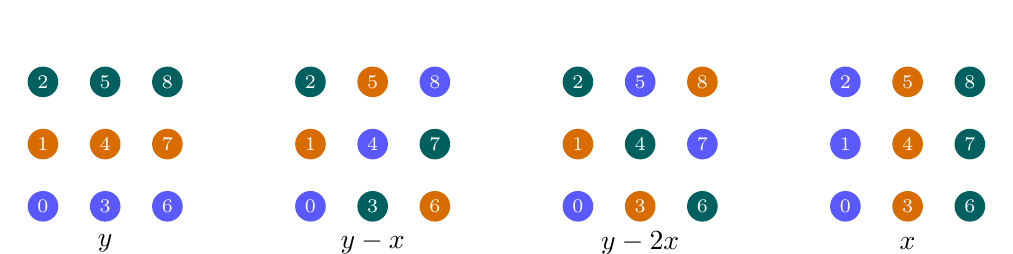
\begin{tikzpicture}[scale=.79]
\foreach \panel in {0,1,2,3}{
 \begin{scope}[xshift=4.3*\panel cm]
 \foreach \x in {0,1,2}{\foreach \y in {0,1,2}{
  \pgfmathtruncatemacro{\lab}{3*\x+\y}
  \ifnum\panel=3\pgfmathtruncatemacro{\cl}{\x}\else
  \pgfmathtruncatemacro{\cl}{mod(\y-\panel*\x+9,3)}\fi
  \ifnum\cl=0\def\clr{blue!65}\else\ifnum\cl=1\def\clr{orange!85!black}\else\def\clr{teal!75!black}\fi\fi
  \fill[\clr] (\x,\y) circle (7pt);
  \node[text=white,font=\scriptsize] at (\x,\y){\lab};
 }}
 \ifnum\panel=0\node at(1,-.6){$y$};\fi
 \ifnum\panel=1\node at(1,-.6){$y-x$};\fi
 \ifnum\panel=2\node at(1,-.6){$y-2x$};\fi
 \ifnum\panel=3\node at(1,-.6){$x$};\fi
 \end{scope}
}
\end{tikzpicture}
\caption{Each color is one final block. Coordinates and colors are interpreted
modulo three. The four plans are tested on the same exact mode-list sizes.}
\label{fig:affine}
\end{figure}

\begin{theorem}[Affine support certificate]\label{thm:affine}
For one operation support $v_j$ chosen from each of the four affine plans,
\[
 \left\|v_1+v_2+v_3+v_4\right\|_2^2\le5400.
\]
Equality is attained by every choice of four final-triangle supports.
Consequently the least-cost plan has local time and local storage coefficient
\begin{equation}
 \beta_9^2=\frac{2\cdot5400}{25\cdot4^2\cdot9^2}
   =\frac13.\label{eq:affine-beta}
\end{equation}
The construction and proof allow arbitrary internal order within each line.
\end{theorem}

\begin{proof}
There are three operation types, with tripartition sizes
$A=(1,1,7)$, $B=(1,2,6)$, and $C=(3,3,3)$. In type $A$ the two singletons
lie on the plan's affine line; in type $B$ the first two parts form that
line. For part sizes $a,b,c$, the largest squared support norm is
\[
 25(ab+ac+bc)-21\min(ab,ac,bc).
\]
The maxima are respectively $354,458,486$, so $\|v_j\|^2\le486$.
We next prove that supports from different directions satisfy $v\cdot w\le288$.

Let $S_v$ be the nonzero support and $D_v$ the discounted subset. If
\[
 c=|S_v\cap S_w|,\quad a=|D_v\cap S_w|,\quad
 b=|D_w\cap S_v|,\quad t=|D_v\cap D_w|,
\]
then
\begin{equation}
 v\cdot w=25c-15(a+b)+9t,\qquad t\le\min(a,b).\label{eq:dot-count}
\end{equation}
The expression $-15(a+b)+9\min(a,b)$ decreases with either $a$ or $b$.
The following elementary counts cover all six type pairs.

For $AA$, each support is all edges incident to two selected collinear
points. Two such pairs on transverse lines are disjoint or meet once.
Their common incident edges number at most nine: the eight edges at the
common point, and the edge between the other two selected points.
Thus the dot product is at most $225$.

For $AB$, enlarge the $B$ support to all edges incident to its entire line.
A transverse two-point set and three-point line have at most ten common
incident edges, giving $250$. For $AC$, the two selected points lie in
different lines of the other parallel class. Each has six crossing
neighbors, with their mutual edge counted twice, so $c=11$ and the bound
is $275$.

For $BB$, two transverse underlying lines meet at $x$. Their full incident
edge sets share twelve edges: eight at $x$ and four between the other two
points on each line. The omitted internal pair edge removes one common
edge unless that operation's singled vertex is $x$. Unless both singled
vertices are $x$, $c\le11$ and the dot product is at most $275$.
If both are $x$, the three possible discounts each meet the common support
in at least two edges. Hence~\eqref{eq:dot-count} gives at most
$300-15(2+2)+9\cdot2=258<275$.

For $BC$, the underlying three-point line meets each line of the other
parallel class once. Of the fifteen crossing edges incident to it, the
$B$ support omits one, so $c=14$. A $C$ discount meets the $B$ support
in at least four edges. A $B$ discount meets the $C$ support in respectively
two, four, or eight edges. Thus the dot product is at most
$350-15(4+2)+9\cdot2=278$.

For $CC$, the two internal-line edge sets are disjoint and each has nine
edges, giving $c=36-9-9=18$. Each discount has six edges crossing the other
partition. The two chosen lines from each direction make a $2$-by-$2$ grid;
its two diagonals are the common discounted edges. Thus $a=b=6,t=2$ and
\[
 v\cdot w=25\cdot18-15\cdot12+9\cdot2=288.
\]
The resulting valid upper table is
\[
\begin{array}{c|rrr}&A&B&C\\\hline
 A&225&250&275\\B&250&275&278\\C&275&278&288
\end{array}
\]
and all entries are at most $288$. Expanding the squared sum now gives
$4\cdot486+2\cdot6\cdot288=5400$.
For four final supports, every individual squared norm is $486$ and every pairwise
dot product is $288$, so equality holds. Lemma~\ref{lem:average} proves
\eqref{eq:affine-beta}.
\end{proof}

This proof establishes a bound for every feasible entropy vector, rather
than sampling random tensor dimensions. The finite checker independently
constructs all supports and verifies the norm and dot-product inequalities.
A separate exhaustive check of all $21^4=194481$ four-tuples gives the same
maximum, with exactly $3^4=81$ maximizers. Their squared norms sum to
$622974240$, an auxiliary reproducibility value.

\subsection{An exact plan selector}
For unordered edge $e=\{g,h\}$ define the positive integer
$d_e=|\mathcal I_{gh}|\,|\mathcal I_{hg}|$. For plan $j$, compute
\begin{equation}
 P_j=\max_{v\in\mathcal V_j}\prod_e d_e^{v_e}.\label{eq:selector}
\end{equation}
Its logarithm is $5F_j(g)$, so choosing the least $P_j$, with fixed-index
tie breaking, chooses the least-cost plan exactly. The number of supports
is fixed; the product bit lengths are polynomial. Empty lists are excluded
before this selector is called. No numerical optimization is executed by
the contraction algorithm.

\section{The other certified menus}
\label{sec:other-menus}

\subsection{A twelve-group certificate with a small combinatorial core}
At the second recursion level use the following four ordered plans:
\begin{center}\small
\begin{tabular}{cl}
\toprule Plan & Final blocks\\\midrule
0 &$(0,1,2,3)\mid(4,5,6,7)\mid(8,9,10,11)$\\
1 &$(9,6,4,0)\mid(1,7,10,11)\mid(5,3,2,8)$\\
2 &$(1,2,10,4)\mid(3,11,6,9)\mid(7,0,8,5)$\\
3 &$(0,5,10,11)\mid(3,8,1,6)\mid(4,9,7,2)$\\
\bottomrule
\end{tabular}
\end{center}
Within each four-point block, merge its first pair and its last pair, then
merge those pairs. The order in the table is part of the certificate.
There are thirty supports per plan, of types $A=(1,1,10)$,
$B=(2,2,8)$, and $C=(4,4,4)$.

\begin{proposition}[Twelve-group bound]\label{prop:twelve}
For these four plans the exact maximum squared sum of supports is
$Q=9864$. Therefore $\beta_{12}^2=137/400$.
\end{proposition}
\begin{proof}
The individual squared-norm maxima are $504,816,864$ for $A,B,C$.
For the six pairs of distinct plans, direct integer counts using
\eqref{eq:dot-count} give the cross-dot upper table
\[
\begin{array}{c|rrr}&A&B&C\\\hline
 A&504&500&400\\B&500&516&500\\C&400&500&540.
\end{array}
\]
This finite table can be verified from the displayed vertex sets, and the
checker reconstructs all six $30$-by-$30$ matrices. If a support tuple has
an internal operation, single it out. Its squared norm is at most $816$ and each
of its three cross dots is at most $516$. The other three squared norms are at
most $864$, with mutual dots at most $540$. Thus the squared norm of the sum is at most
\[
 816+3\cdot864+2(3\cdot516+3\cdot540)=9744.
\]
It remains to examine the three final supports in each plan. Index them
by their discounted class, in order $(0,1),(0,2),(1,2)$. Their pairwise
dot product is $540$ when $x_j=p_{ij}(x_i)$ and $522$ otherwise, where
\[
\begin{array}{c|rrrrrr}
 ij&01&02&03&12&13&23\\\hline
 (p_{ij}(0),p_{ij}(1),p_{ij}(2))
 &(1,2,0)&(1,0,2)&(2,0,1)&(0,2,1)&(1,2,0)&(2,1,0).
\end{array}
\]
These six tiny matrices are also checked directly. Triangles $012,023,123$
are inconsistent: for every $x$, $p_{jk}(p_{ij}(x))\ne p_{ik}(x)$.
Only triangle $013$ is consistent. Five edges of $K_4$ contain two
triangles, so five preferred relations cannot hold at once. At most four
pairs have dot $540$, and four are attained at $(x_0,x_1,x_2,x_3)=(0,1,0,2)$.
Consequently
\[
 Q=4\cdot864+2(6\cdot522+4\cdot18)=9864>9744.
\]
Finally $2Q/(25\cdot4^2\cdot12^2)=137/400$.
\end{proof}
The certificate was suggested by a finite search. Its validity depends only
on the four displayed plans and the exact checks, not on the search or its
floating-point heuristic. Independent enumeration of all $30^4=810000$
tuples gives nine maximizers and squared-norm sum $3501532800$.
No global optimality over other menus is asserted.

\subsection{Puncturing the affine plane and ending the recursion}
Delete point $8$ from every affine block to obtain the eight-group menu.
Delete points $7,8$ for the seven-group menu. Keep the surviving order and
use the same balanced split rule. No block is empty. Direct exact support
certificates give
\begin{center}
\begin{tabular}{rrrrrl}
\toprule $r$ & Plans & Supports/plan & Tuples & $Q$ & $\beta_r^2$\\\midrule
9 &4&21&194481&5400&$1/3$\\
12&4&30&810000&9864&$137/400$\\
8 &4&18&104976&4464&$279/800$\\
7 &4&15&50625&3564&$891/2450$\\
4 &1&6&6&104&$13/25$\\
\bottomrule
\end{tabular}
\end{center}
The four-group plan is simply $(0,1)\mid(2)\mid(3)$. Its two operations
both have tripartition sizes $(2,1,1)$, up to ordering, and the largest
squared support norm is $104$. The punctured certificates are finite
integer exhaustions, not extrapolations of the nine-point geometry.
The independently reconstructed sums for $r=8,7$ are respectively
$289547136$ and $118219500$.

The compact certificate theorem improves the menu coefficients within the
current mode-entropy model. It does not assert that every algebraic entropy
vector is realized by a SAT instance, that the chosen tree is globally
optimal, or that tensor contraction requires explicit tables in every
possible representation.

% Standalone section fragment. Requires amsmath, amssymb, amsthm, booktabs.
\section{A fully paid rational recursion with five group counts}
\label{sec:schedule}

This section assumes the reviewed normalized contraction interface, rather
than claiming an independent proof of the upstream SAT reduction. Let $s$
be the root wire count, $\mathcal L$ the input-description length, and
$\lambda=\lceil\log_2s\rceil$. The root maximum degree is at most
$\lceil s^{9/10}\rceil$; initial precision and truncation order are at most
$s$. The imported entry-evaluation, creation-precision, padding, exact
Cauchy-mode factorization, and Hermite recovery contracts are unchanged.

For the group counts used below, the certified local aggregation coefficients
are
\[
 b_9^2=\frac13,\quad b_{12}^2=\frac{137}{400},\quad
 b_8^2=\frac{279}{800},\quad b_7^2=\frac{891}{2450},\quad
 b_4^2=\frac{13}{25}.
\]
The first is the four-direction affine-plane certificate. The next is the
fixed four-plan twelve-group certificate; the eight- and seven-group
certificates are punctured affine portfolios. The final coefficient uses
one tree with final blocks $(0,1)\mid(2)\mid(3)$: its largest squared
undirected support norm is $104$, hence $b_4^2=2(104)/(25\cdot4^2)$.
Each coefficient simultaneously bounds local aggregation work and local
storage, including the singleton factor tables. No matrix algorithm beyond
the already imported $\omega<12/5$ bridge is needed.

\subsection{All recursive factor calls are charged}

Put
\[
 \kappa=\frac{\pi\sqrt2}{\ln2},\qquad
 K_d=\kappa\frac{M_d}{\sqrt{u_d}},\qquad
 \alpha_r=\frac{\sqrt{2(r-1)}}r.
\]
Each singleton factor is incident with $2(r-1)$ directed pair indices.
Applying the inherited weighted pair-entropy inequality to this indicator
vector bounds its number of entries by
$2^{(\alpha_r+o(1))K_d}$. Every entry invokes the actual child contraction.
Enumerating all exact pair-budget arrays has only polynomial cost because
$r\le12$ is fixed and all budgets are polynomial in $s$. Consequently the
fully paid time recurrence is
\begin{equation}\label{eq:new-paid-recurrence}
 T_d\le\operatorname{poly}(s)
 \left(2^{(\alpha_{r_d}+o(1))K_d}T_{d+1}
       +2^{(b_{r_d}+o(1))K_d}\right).
\end{equation}
The local storage bound is a polynomial factor times
$2^{(b_{r_d}+o(1))K_d}$. Uniform input access contributes one fixed
polynomial factor in $s+\mathcal L$ to the full algorithm: count arithmetic
and entry requests first, and then charge their uniform description-access
cost. It is not necessary to multiply an input-description polynomial anew
at each recursion level.

\subsection{The strict rational schedule}

Use the group sequence
\[
 (r_0,r_1,r_2,r_3,r_4,r_5,\ldots)=(9,12,8,7,4,4,\ldots)
\]
and taper fractions
\begin{align*}
 \eta_0&=\frac{63}{4000},&
 \eta_1&=\frac{97}{8000},&
 \eta_2&=\frac{21}{4000},&
 \eta_3&=\frac{31}{12500},\\
 \eta_d&=\frac{106449}{20000000}
             \left(\frac{63}{100}\right)^{d-4}\quad(d\ge4).
\end{align*}
Let
\[
 u_d=\lfloor\eta_d\lambda\rfloor,\qquad
 B=\lceil6\log_2\lambda\rceil,\qquad
 a_d=\sum_{j=0}^d u_j+(d+1)B,
 \quad L_d=2^{a_d},\quad Q_d=r_d^{a_d}.
\]
The tail fractions sum to $2877/200000$, and
\begin{equation}\label{eq:new-total-retention}
 \sum_{d\ge0}\eta_d=\frac{4999}{100000}<\frac1{20}.
\end{equation}
Use direct contraction when $M\le H=\lceil s/\lambda^{3/4}\rceil$.
A finite exceptional range in $s$ can also be handled directly. Choose
padding slack $\lambda^{-3}$, as allowed by the unchanged packing interface.

\subsection{Packing gates and the depth bootstrap}

At the root, a sufficient gate is $Q_0^2\Delta/M=o(1)$, up to fixed
polylogarithmic factors. Below the root the sufficient gates are
\[
 Q_dR/M=o(1),\qquad
 Q_d^2C\operatorname{polylog}(s)/M=o(1),\qquad
 L_dQ_d^2/M=o(1),
\]
where $R\le\Delta\le s^{9/10+o(1)}$ and
$C\le2L_{d-1}$. The latter bound is the imported retained-side/fresh-side
invariant, not an assumption that all descendants have bounded degree.

The exact integer inequalities
\[
 9^{100}<2^{317},\quad 12^{200}<2^{717},\quad
 7^{5000}<2^{14037}
\]
give the required rational logarithm upper bounds. Using them, the gaps
below exponent one in the dominant gates are
\[
\begin{array}{c|ccccc}
 \text{stage}&0&1&2&3&d\ge4\\ \hline
 \text{gap}&29/200000&109/1600000&1/1600&
 42523/1000000000&1/50000.
\end{array}
\]
The root row uses $2\eta_0\log_2 9+9/10$; the other rows use the cumulative
retained fraction times $\log_2r_d$, plus $9/10$.
For the fresh-side and packet gates it suffices uniformly to use
\[
 \left(1+2\cdot\frac{717}{200}\right)
       \frac{4999}{100000}
 =\frac{4084183}{10000000}<1.
\]
The old packet side contributes no larger exponent than the total retained
fraction. Every fresh degree is at most $s^{4999/100000+o(1)}$, so it remains
below $\Delta$.

Here is a noncircular depth argument. Consider hypothetical active depths
up to $\lceil(3/4)\log_{20/11}\lambda\rceil+O(1)$ and suppose $M>H$.
Because the tail ratio $63/100$ exceeds $11/20$, its taper is at least
a fixed positive constant times $\lambda^{1/4}$ throughout this range.
The guard contributes $O((\log\lambda)^2)$ to every $a_d$. The strictly
positive gaps above absorb these guards, all packing polylogarithms, and
$s/M\le\lambda^{3/4}$ uniformly. Thus padding has relative error
$O(\lambda^{-3})+s^{-c+o(1)}$ for some fixed $c>0$. Every child has size
$(2/r_d+o(1))M\le(11/20)M$ eventually. An active path therefore cannot
reach beyond the hypothetical range. This closes the depth induction and
establishes that all active tapers diverge. Their floors have relative
$o(1)$ error.

The product of padding errors over $O(\log\lambda)$ levels is $1+o(1)$.
Hence the child-size bounds are
\[
 M_0\le s,\quad M_1\le(1+o(1))\frac{2s}{9},\quad
 M_2\le(1+o(1))\frac{s}{27},\quad
 M_3\le(1+o(1))\frac{s}{108},
\]
and
\[
 M_{4+j}\le(1+o(1))\frac{s}{378\,2^j}\qquad(j\ge0).
\]

\subsection{Precision and entry costs}

For retained valuations $i<u_d$ the deformation scale obeys
$D=2^{a_d-i}\ge2^{a_{d-1}+B+1}$, with the evident root convention.
The imported creation-time precision bound
$p=O(s\lambda^2 2^{a_{d-1}})$ therefore satisfies
\[
 \frac{p}{MD/u_d}=O(\lambda^{15/4}2^{-B})=o(1).
\]
The remaining additive Hermite loss is lower order for the same reason.
Thus the sharp local evaluation precision
$p_t\le(6+o(1))MD/u_d$ and the weighted entropy estimates hold uniformly.
All ring ranks, coordinate bit lengths, and exact budgets are polynomial
in $s$, since $a_d\le(4999/100000)\lambda+O((\log\lambda)^2)$.

Direct leaf work is $2^{O(s/\lambda^{3/4})}$. Original entry routines cost
$2^{O(s^{9/10})}$ times a polynomial, and fresh entry routines cost at most
$\exp(s^{4999/100000+o(1)})$. Each is lower order on the scale
$s/\sqrt\lambda$. Creation-time tensor descriptions remain immutable;
no earlier contraction algorithm is recursively expanded inside a fresh
entry routine. The multiplicities of all entry and child calls are already
included in \eqref{eq:new-paid-recurrence}.

\subsection{Exact time and space constants}

Write
\[
 (m_0,m_1,m_2,m_3,m_4)=\left(1,\frac29,\frac1{27},
                                     \frac1{108},\frac1{378}\right),
 \qquad K_i^*=\frac{\kappa m_i}{\sqrt{\eta_i}}\quad(0\le i\le4).
\]
Successive tail coefficients have ratio
\[
 \gamma=\frac{1/2}{\sqrt{63/100}}=\frac5{\sqrt{63}}<1.
\]
Let $P_j=\sum_{i<j}\alpha_{r_i}K_i^*$. Unrolling the paid recurrence gives
four finite-prefix candidates $P_j+b_{r_j}K_j^*$ for $0\le j\le3$, and the
whole tail is bounded by
\[
 C_\infty=P_4+K_4^*
       \max\left\{b_4,\frac{\alpha_4}{1-\gamma}\right\}.
\]
Indeed a tail aggregation at offset $t$ has exponent coefficient
\[
 P_4+K_4^*\left(
 \frac{\alpha_4}{1-\gamma}(1-\gamma^t)+b_4\gamma^t\right),
\]
a convex combination of the two endpoint coefficients. Here
$\alpha_4/(1-\gamma)>b_4$, so the infinite leaf-route sum bounds every
finite tail operation.

Exact rational outward intervals give the following certified values:
\[
\begin{array}{c|l}
 \text{branch}&\text{coefficient, shown to 12 decimal places}\\ \hline
 0&29.487537286921\\
 1&30.269872910441\\
 2&29.690498000478\\
 3&30.006711339131\\
 \infty&30.262408169228.
\end{array}
\]
The second row dominates. Thus
\begin{equation}\label{eq:new-time-constant}
 C_T=\frac{\pi}{\ln2}\left(
        \sqrt{\frac{128000}{5103}}+
        \sqrt{\frac{21920}{7857}}\right)
 =30.269872910441123\ldots<30.27.
\end{equation}
Fixed polynomial overheads across $O(\log\lambda)$ depths add only
$O(\lambda\log\lambda)=o(s/\sqrt\lambda)$ to the logarithmic running time.

Ancestor tables coexist by addition of storage sizes, rather than by
multiplication. The local memory coefficients at the five first occurrences
are respectively
\[
 \begin{array}{ccccc}
29.487537286921\ldots & 7.570356123317\ldots & 1.934875839854\ldots \\
0.718696654792\ldots & 0.167607514679\ldots
\end{array};
\]
later ones decrease geometrically. Therefore
\begin{equation}\label{eq:new-space-constant}
 C_S=\frac{\pi}{\ln2}\sqrt{\frac{8000}{189}}
 =29.487537286921217\ldots<29.488.
\end{equation}
The resulting normalized contraction has bit time
\[
 (s+\mathcal L)^{O(1)}2^{(C_T+o(1))s/\sqrt{\log_2s}}
\]
and bit space
\[
 (s+\mathcal L)^{O(1)}2^{(C_S+o(1))s/\sqrt{\log_2s}}.
\]
This improves the explicit normalized upper-bound pair
$30.891018920366\ldots/30.753912832055\ldots$ from the newest prior
three-plan certificate. It uses subexponential space. It neither changes
the logarithmic order of the exponent nor identifies the wire count $s$
with the number of SAT variables.

The accompanying standard-library checker proves rational logarithm gates
by integer powers, encloses $\pi$ by Machin's alternating series and
$\ln2$ by its positive atanh series, encloses all square roots by integer
square roots, and rejects the unsupported time coefficient $30.26$ and two
invalid precision schedules. It checks a finite arithmetic certificate;
it is not a formal proof of the imported interfaces or a full SAT solver.

\section{An exact Toeplitz kernel for packet actions}
\label{sec:kernel}

This section gives a second, independent improvement: a faster exact
\emph{matrix--vector subroutine}. It does not change the entropy coefficient
or the logarithmic order of the SAT bound. Toeplitz multiplication and
Kronecker substitution are classical; the contribution relative to the
reviewed corpus is the ring-safe packet specialization, its implementation,
and its comparison with an appropriate Boolean-input control.

\subsection{The convolution identity}
In the source packet deformation~\cite{openai}, let $L=2^a$,
$S=\{-L,\ldots,L-1\}$, $\alpha=2L$, and
\[
 C(T)=\prod_{q\in S}(T-q),\qquad T=t+\alpha\zeta,\quad t\in S.
\]
For $-L<d<L$, define the cancelled polynomial
\[
 w_d=\frac{\prod_{q\in S\setminus\{d\}}(T-q)}{C'(0)}.
\]
The inherited integrality statement makes these entries meaningful in the
source coefficient ring. The packet matrix satisfies
$W_{xy}=w_{y-x}$ for $0\le x,y<L$ and is therefore Toeplitz. Put
\[
 A(X)=\sum_{d=-L+1}^{L-1}w_dX^{d+L-1},\qquad
 B(X)=\sum_{y=0}^{L-1}v_yX^{L-1-y}.
\]
Then the exact identity
\begin{equation}
 (Wv)_x=[X^{2L-2-x}]A(X)B(X)\label{eq:toeplitz}
\end{equation}
holds over every commutative coefficient ring. Zero-fill excluded columns
and discard excluded rows to obtain a masked action. For rows $r+hj$ and
columns $c+hk$, use the shorter Toeplitz kernel
$w_{c-r+h(k-j)}$. In particular, opposite parity masks use dimension $L/2$.
No Fourier transform, inverse of $L$, or division by a nonunit is required.

\subsection{Integral diagonal preparation}
The delivered implementation fixes
\[
 R_p=(\mathbb Z/2^p\mathbb Z)[U]/(U^2+U+1).
\]
It accepts exact integer coordinates of $\zeta$ before reducing the output.
Since $U^2+U+1$ is irreducible modulo two, an element is a unit precisely
when its two integer coordinates are not both even. Its valuation is the
minimum of their two-adic valuations.

For $d\ne t$, $v_2(T-d)=v_2(t-d)\le a$. If $\zeta\ne0$, the remaining
factor has valuation $a+1+v_2(\zeta)$. The complete residue grid gives
\[
 \sum_{q\in S\setminus\{t\}}v_2(t-q)=v_2(C'(0)),\qquad
 v_2(C(T)/C'(0))=a+1+v_2(\zeta).
\]
Cancelling any one factor leaves a nonnegative valuation. Split each exact
factor into a power of two and a unit before modular reduction. Multiply
the units, cancel the odd part of $C'(0)$, and batch-invert all factor units.
Restore only the nonnegative final power of two. The inverse identity is
\[
 (a+bU)^{-1}=\frac{(a-b)-bU}{a^2-ab+b^2};
\]
the denominator is odd for a unit. Preparation uses $O(L)$ ring operations
and two unit inversions. Arbitrarily long input coordinates incur their
own reading and normalization cost.

If $\zeta=0$, cancel the unique zero factor symbolically: only $w_t$ can
survive, and it is $C'(t)/C'(0)$. If $t=-L$, that diagonal is outside the
matrix and the action is zero. These cases are explicitly implemented.

\subsection{Exact integer convolution and bit cost}
For nonnegative coordinate arrays $(a_i),(b_j)$, every ordinary convolution
coefficient is at most $\min(\#a,\#b)(\max a_i)(\max b_j)$. Choose a
byte-aligned power of two $Q$ strictly larger than this bound, pack the
arrays as $\sum_i a_iQ^i$ and $\sum_jb_jQ^j$, multiply integers, and unpack.
No digit can carry into its neighbor. Reduce the extracted coefficients
modulo $2^p$. Byte-array packing avoids repeated large-integer shifts.

For coordinate arrays $a+bU$ and $c+dU$, three scalar convolutions suffice:
\[
 A=a*c,\quad B=b*d,\quad C=(a+b)*(c+d),\qquad
 (a+bU)*(c+dU)=(A-B)+(C-A-2B)U.
\]
A Boolean input uses just the two coordinate convolutions with that input.
Let $M_{\rm int}(b)$ denote the bit cost of multiplying $b$-bit integers,
and $I(p)$ that of a unit inversion at precision $p$. After input
normalization, a conservative bound for preparation plus application is
\begin{equation}
 O\!\left(LM_{\rm int}(p+\log L)+I(p)
              +M_{\rm int}(L(p+\log L))\right).\label{eq:kernel-cost}
\end{equation}
This includes reading and writing the full vector. Working storage for
the action is $O(L(p+\log L))$ bits, in addition to whatever workspace the
chosen integer multiplier needs. With a quasi-linear, near-linear-space
integer multiplier the action is quasi-linear in the packed input size.
The Python prototype uses its host's big-integer multiplication; it does
not implement an asymptotically optimal multiplier.

The Toeplitz identity also holds for unramified extension degree $e$ and
nilpotent length $\ell$. Because $W$ has no $V$ dependence, a conservative
coordinate extension needs $e^2\ell$ scalar convolutions plus polynomial
coefficient reduction. That extension is an algorithmic observation, not
an implemented arbitrary-ring interface in this archive.

\subsection{Matched controls, including the negative result}
The independent diagonal oracle forms each cancelled product at extra
precision and only then removes the known power of two. It shares neither
the batch-inversion preparation nor the convolution algorithm. The action
oracle performs literal matrix--vector summation. For Boolean input, a
stronger control skips zero columns and masked rows and uses additions
only. This matters: multiplication-heavy dense controls overstate a speedup
for the actual Boolean special case.

Five-repeat synthetic timings are retained in
\texttt{results/benchmarks.json}. Ratios below are control time divided by
new time; a ratio below one means the new routine is slower. The general
column includes preparation on both sides. Boolean columns measure action
only with the same prepared diagonals.
\begin{center}\small
\begin{tabular}{rr rrr}
\toprule $L$ & $p$ & General, incl. preparation & Boolean full grid & Boolean strided\\\midrule
32&32&1.656&0.178&0.332\\
64&64&2.432&0.208&0.427\\
128&64&4.123&0.324&0.691\\
256&128&4.434&0.345&0.846\\
512&128&6.643&0.491&1.272\\
1024&128&---&0.772&2.013\\
\bottomrule
\end{tabular}
\end{center}
Thus the generic convolution loses to the stronger Boolean control on
every sampled fixture. The strided specialization wins only at the two
largest sampled sizes. This is useful implementation evidence, not a
measured SAT improvement. The coefficient theorem of the preceding section
does not rely on these timings or on this kernel.

\section{What would change the logarithmic order?}
\label{sec:research}

The geometric menu removes a genuine bottleneck in the submitted
constant calculation. It does not remove the partition-growth mechanism
that produces the square root of the logarithm. It is useful to identify
the remaining task precisely, and to separate it from optimizations that
can only improve constants under the present interface.

\subsection{The alternative crossing interface in the public paper}
Anthropic's Appendix A gives a general crossing-piece construction with
a parameter $\rho$. A polynomial-size family of exact crossing pieces
whose row and column factorization bit counts sum to
\[
 4\rho\lambda+O(\log\lambda)
\]
gives logarithmic denominator power $\log_2(1/\rho)$. Appendix B realizes
$\rho=1/\sqrt2$ using a graded Heisenberg representation and ordinary
partition growth~\cite{anthropic-paper}. The full interface includes exact
arithmetic size, piece construction, entry evaluation, and an adaptive
choice of the cheaper row or column aggregation.

Appendix H already identifies the following research direction: a compatible
representation with
\[
 \log\dim V_E\asymp E^\alpha
\]
would suggest $\rho=2^{\alpha-1}$ and hence logarithmic denominator power
$1-\alpha$. This observation belongs to that source. A representation with
$\alpha<1/2$ would be a promising route to an order improvement \emph{if}
it also supplied all exact operator identities, locality, coefficient-size
bounds, and effective evaluation guarantees. A small graded dimension by
itself does not supply those properties.

The most useful research target after this review is therefore an exact,
efficiently evaluable two-sided crossing decomposition with
$\rho<1/\sqrt2$, or an equally explicit replacement for the Cauchy
weighted-mode interface. We do not construct either object here.

\subsection{Why merely keeping square-indexed oscillators fails}
The reviewed earlier second-round note already warned that assigning square
weights to the oscillator modes breaks the necessary degree closure
\cite{degree-barrier}. A different tempting change is to delete all
nonsquare modes. It does improve a bare dimension count, but has a simple
locality obstruction.

Let $p_\square(E)$ be the number of partitions of $E$ into square parts.
Then
\[
 \log p_\square(E)=\Theta(E^{1/3}).
\]
For a lower bound, choose arbitrary subsets of
$2^2,3^2,\ldots,J^2$ with $J=cE^{1/3}$ for a sufficiently small fixed
$c>0$, and fill the remaining weight with ones. For an upper bound, use
the generating function and the Gaussian sum:
\begin{align*}
 \log p_\square(E)
 &\le\theta E+\sum_{k\ge1}\frac1k\sum_{j\ge1}e^{-\theta k j^2}\\
 &\le\theta E+O(\theta^{-1/2});
\end{align*}
take $\theta=E^{-2/3}$. This numerical growth improvement is not enough.

\begin{proposition}[A scoped finite-pole obstruction]
Let $S$ be an infinite set of positive integers with arbitrarily long gaps,
and put $a_m=m$ when $|m|\in S$ and $a_m=0$ otherwise. The restricted
scalar Heisenberg-current commutator
\[
 C_S(z,w)=\sum_{m\in\mathbb Z}a_m z^{-m-1}w^{m-1}
\]
is not annihilated by $(z-w)^H$ for any finite nonnegative integer $H$.
\end{proposition}
\begin{proof}
If that product vanished, coefficient comparison would give
\[
 \sum_{j=0}^H(-1)^j\binom Hj a_{n-j}=0
 \quad\text{for every integer }n.
\]
For $H>0$, $H$ consecutive zero values would force all later values to be
zero by this recurrence. An arbitrarily long gap followed by another
element of $S$ is a contradiction. The case $H=0$ is immediate.
For square indices, there is the explicit witness
$n=(H+1)^2$: all preceding $H$ indices are nonsquares, and the displayed
coefficient equals $n\ne0$.
\end{proof}
This blocks the naive deletion of oscillator modes in the current used
by the source construction. It is not a lower bound against all vertex
algebras, all sparse gradings, all crossing decompositions, or all SAT
algorithms. The included finite witness program is a check on the formula;
the proposition itself is an all-size proof.

\subsection{Further constant improvements and their limit}
The support-averaging problem has an independent finite-geometric form.
One seeks menus for which the sums of all possible operation supports
have small Euclidean norm. The affine-plane construction works because
different parallel classes are transverse, and this controls every
intermediate support as well as the final triangle. It is reasonable to
search other designs or weighted mixtures of plans. However, the coefficient
we prove is a valid certificate for the supplied menu, not a proof that
the menu or the rational schedule is globally optimal.

A pointwise cheapest-plan bound can also be strictly better than the
uniform arithmetic average used by Lemma~\ref{lem:average}. Establishing
that improvement would require a new uniform bound on
$\min_j\max_{v\in\mathcal V_j}v\cdot g$ over the admissible nonnegative
entropy vectors. Numerical optimization without a rigorous certificate
would not justify a stronger constant. Likewise, letting the group count
grow with input size requires controlling the number of budget allocations,
all pair directions, packet packing, and table construction uniformly;
our fixed-$r$ proof does not do so.

The twelve-group menu was found by finite search and then certified
independently. Its validity depends only on the frozen plans and the
integer certificate. Replaying the search is not necessary to verify the
result. No negative search result in this report is promoted to an
impossibility theorem.

\section{Verification, artifacts, and integration}
\label{sec:repro}

\subsection{What the certificate programs actually establish}
All delivered correctness checkers use only the Python standard library.
They use explicit exceptions rather than Python assertions, so their
checks remain active under \texttt{python3 -O}. Normal and optimized
executions produce identical JSON for every checker.
\begin{center}\small
\begin{tabular}{p{4.4cm}p{9.5cm}}
\toprule Checker & Evidence and scope\\\midrule
\texttt{check\_portfolios.py}&Exhaustive integer support norms for all five
group counts; compact geometric/twelve-group certificates; 100 exact plan
selection cases; deliberate rejection of a false $Q=9863$.\\
\texttt{check\_schedule.py}&Integer logarithm certificates, rational outward
intervals for $\pi$, $\ln2$, square roots and every paid branch; strict
packing gates; invalid taper/tail and $30.26$ negative controls.\\
\texttt{check\_affine\_algebra.py}&45 fixtures, 153 complete planned
contractions, 749 literal assignments, and 3,013 paid group-entry calls
over $(\mathbb Z/64\mathbb Z)[V]/(V^2)$.\\
\texttt{check\_toeplitz.py}&1,048 packet cases; 12,328 independent cancelled
diagonals; 2,096 general actions; 149 masked actions; 1,048 Boolean and
1,048 strided actions; 350 unrelated convolutions; 10 invalid inputs.\\
\texttt{check\_lacunary.py}&Explicit nonzero finite-difference witnesses
for pole orders $0$ through $64$.\\
\bottomrule
\end{tabular}
\end{center}
The algebra test caches every singleton factor and compares the full plan
with a literal graphical sum. Its oracle expands constant and linear
coefficients directly rather than sharing the evaluator's ring
multiplication. Fixtures include zero divisors, nilpotents, distinct
opposite orientations, singleton dimensions, empty allocations, and
disconnected effective graphs. The finite implementation uses literal
rectangular multiplication; the theoretical fast matrix backend is a
separate inherited existence argument.

These tests corroborate the implementation and the finite certificates.
They do not prove the all-size packing and recovery interfaces, run a full
SAT solver, or constitute Lean verification of the new theorem. The
all-size additions in this report are justified by the mathematical
arguments, with the proof dependencies stated explicitly.

\subsection{Replaying the package}
From the extracted archive directory, run
\begin{lstlisting}
python3 code/run_checks.py
python3 code/verify_manifest.py
bash build.sh
\end{lstlisting}
The first command runs every checker normally and with optimization,
compares outputs, and writes a combined verification report. The second
checks file integrity against the packaged manifest. The third builds
\texttt{report.pdf} from the included \LaTeX{} sources; it needs a normal
TeX installation with \texttt{latexmk}, AMS packages, TikZ, and Latin Modern.
Recorded benchmark timings are evidence from this session, not deterministic
test expectations. To measure them again, use
\begin{lstlisting}
python3 code/check_toeplitz.py --benchmark --output benchmarks_rerun.json
\end{lstlisting}

\subsection{Contents and proof status}
The archive includes the complete \LaTeX{} source tree and compiled PDF;
frozen contraction menus; exact certificate and algebra programs; normal
and optimized JSON results; raw benchmark samples; a source review and
independent audit notes; immutable source URLs and hashes; and a
machine-readable \texttt{PROOF\_STATUS.json}.

The source provenance identifies both repositories at exact commits and
all nine incoming ZIP hashes. Primary upstream source files are not
duplicated wholesale. The package is self-contained for replaying its
new finite certificates and for building its PDF; reading the inherited
proofs requires the referenced source snapshots.

For repository integration, this is a proposed new research packet. No
remote branch, issue, pull request, or repository file was changed during
this session. The latest repository documentation already records that the
Anthropic formalization is public at the supplied revision. The new
numerical frontier here is a separate normalized contraction theorem.

\begin{thebibliography}{20}
\small
\bibitem{openai} OpenAI, \emph{The Exponential Time Hypothesis is False},
October 25, 2026, quantitative contraction/reduction source, revision
\texttt{7ef5c0cc5ca4b0e072b7a050fca09ab24bc6fa3a}.
\href{https://github.com/openai/math/tree/7ef5c0cc5ca4b0e072b7a050fca09ab24bc6fa3a/preprints/The-Exponential-Time-Hypothesis-is-False-October-25-2026}{Immutable source link}.

\bibitem{tree} ProveIt incoming packet,
\emph{sat\_adaptive\_tree\_certificate\_2026-10-26.zip},
in the reviewed snapshot. Internal sources include its report,
finite support certificates, and paid-schedule proof.
\href{https://github.com/VladimirReshetnikov/ProveIt/blob/73dfb5e5ab6e91bd7375e5b97ef85d7e1cc8e81d/docs/incoming/sat_adaptive_tree_certificate_2026-10-26.zip}{Immutable source link}.

\bibitem{flags} ProveIt incoming packet,
\emph{sat\_adaptive\_bounds\_2026-10-26.zip}.
\href{https://github.com/VladimirReshetnikov/ProveIt/blob/73dfb5e5ab6e91bd7375e5b97ef85d7e1cc8e81d/docs/incoming/sat_adaptive_bounds_2026-10-26.zip}{Immutable source link}.

\bibitem{asymmetric} ProveIt filed packet,
\emph{eth\_asymmetric\_packet\_balancing}, report and proof status.
\href{https://github.com/VladimirReshetnikov/ProveIt/tree/73dfb5e5ab6e91bd7375e5b97ef85d7e1cc8e81d/Computability/SubexponentialSAT/Research/eth_asymmetric_packet_balancing}{Immutable source link}.

\bibitem{joint} ProveIt filed packet,
\emph{eth\_joint\_cauchy}, full-block Cauchy mode entropy.
\href{https://github.com/VladimirReshetnikov/ProveIt/tree/73dfb5e5ab6e91bd7375e5b97ef85d7e1cc8e81d/Computability/SubexponentialSAT/Research/eth_joint_cauchy}{Immutable source link}.

\bibitem{tree-old} ProveIt filed packet,
\emph{subsat\_contraction\_tree}, exact ring matrix aggregation and
tree-support method.
\href{https://github.com/VladimirReshetnikov/ProveIt/tree/73dfb5e5ab6e91bd7375e5b97ef85d7e1cc8e81d/Computability/SubexponentialSAT/Research/subsat_contraction_tree}{Immutable source link}.

\bibitem{degree-barrier} ProveIt filed packet,
\emph{3sat\_round2\_refinement},
\texttt{research\_alternate/}\allowbreak
\texttt{heisenberg\_entropy\_barrier.md}.
\href{https://github.com/VladimirReshetnikov/ProveIt/blob/73dfb5e5ab6e91bd7375e5b97ef85d7e1cc8e81d/Computability/SubexponentialSAT/Research/3sat_round2_refinement/research_alternate/heisenberg_entropy_barrier.md}{Immutable source link}.

\bibitem{anthropic-pr} Anthropic, \emph{formal-math}, pull request 31,
user-supplied revision \texttt{1a6eee293b9e00cb432eef6018a21f523623a9af}.
\href{https://github.com/anthropics/formal-math/pull/31/changes/1a6eee293b9e00cb432eef6018a21f523623a9af}{Immutable source link}.

\bibitem{anthropic-statement} Anthropic,
\texttt{eth/MainResults.lean}, \texttt{Solution.lean},
\texttt{README.md}, and \texttt{comparator.json}, supplied revision.
\href{https://github.com/anthropics/formal-math/tree/1a6eee293b9e00cb432eef6018a21f523623a9af/eth}{Immutable source link}.

\bibitem{anthropic-paper} Anthropic,
\texttt{eth/paper.pdf}, supplied revision, especially Appendices A, B, H.
\href{https://github.com/anthropics/formal-math/blob/1a6eee293b9e00cb432eef6018a21f523623a9af/eth/paper.pdf}{Immutable source link}.

\bibitem{mm} Josh Alman, Ran Duan, Virginia Vassilevska Williams,
Yinzhan Xu, Zixuan Xu, and Renfei Zhou,
\emph{More Asymmetry Yields Faster Matrix Multiplication},
arXiv:2404.16349. Only the conservative consequence $\omega<12/5$
is used here. \href{https://arxiv.org/abs/2404.16349}{Immutable source link}.
\end{thebibliography}

\end{document}
